\documentclass{acm_proc_article-sp}
%\documentclass{sig-alternate}
\usepackage[latin1]{inputenc}
\usepackage{amsmath}
\usepackage{amsfonts}
\usepackage{amssymb}
\usepackage{graphicx}
\usepackage{listings}
\usepackage{url}
\usepackage{havannah}
\usepackage{enumitem}

\newcommand{\hblack}{\texttt{Black}}
\newcommand{\hwhite}{\texttt{White}}
\newcommand{\hblacks}{\texttt{Black's}}
\newcommand{\hwhites}{\texttt{White's}}
\newcommand{\loc}[1]{\texttt{#1}}

\title{Evolutionary Learning of Policies for MCTS Simulations}
\numberofauthors{2}
\author{ 
% 1st. author
\alignauthor
James Pettit \\
       \affaddr{U.C. Santa Cruz}\\
       \affaddr{Santa Cruz, California}\\
       \email{ jpettit@soe.ucsc.edu}
% 2nd. author
\alignauthor
David Helmbold \\
       \affaddr{U.C. Santa Cruz}\\
       \affaddr{Santa Cruz, California}\\
       \email{dph@soe.ucsc.edu}
}

\begin{document}

\toappear{Permission to make digital or hard copies of all or part of this work for
   personal or classroom use is granted without fee provided that copies are
   not made or distributed for profit or commercial advantage and that copies
   bear this notice and the full citation on the first page. To copy otherwise,
   to republish, to post on servers or to redistribute to lists, requires prior
   specific permission and/or a fee. \\
   FDG '12, May 29-June 1, 2012 Raleigh, NC, USA. \\
   Copyright (c) 2012 ACM 978-1-4503-1333-9/12/05... \$10.00.}

\maketitle

\setlist{topsep=0.5pt,partopsep=0.5pt,parsep=0.5pt,itemsep=0.5pt}

\begin{abstract}
Monte-Carlo Tree Search (MCTS) 
grows a partial game tree and uses a large number of random simulations to
approximate the values of the nodes.   
It has proven effective in games with such as Go and Hex where the large search space and
difficulty of evaluating positions cause difficulties for standard methods.
The best MCTS players use carefully hand-crafted rules to bias the random simulations.
Obtaining good  hand-crafting rules is a very difficult process, as even rules promoting better
simulation play can result in a weaker MCTS system~\cite{gelly2006modification}.
Our Hivemind system uses evolution strategies to automatically learn effective rules for biasing the 
random simulations.
We have built a MCTS player using Hivemind for the game Hex. 
The Hivemind learned rules result in a 90\% win rate against a baseline MCTS system, and 
significant improvement against the computer Hex world champion, MoHex.
\end{abstract}

\category{I.2.6}{Computing Methodologies}{Artificial Intelligence}

\keywords{Monte Carlo Tree Search, Computer Hex, Evolution Strategies, Evolutionary Learning, Adversarial Search, Monte Carlo} 

\section{Introduction}

Abstract strategy games provide an attractive testbed for artificial intelligence and machine learning applications. The game framework provides immediate feedback on algorithm performance. 
Starting with mathematical game theory research, the most common technique for game AI has been brute force search of the tree of legal moves. 
This technique, highly tuned and optimized, is what led to Chinook's ascendance to World Champion in 1994 and Deep Blue's eventual victory in 1997 over then World Champion Gary Kasparov. These victories cemented brute force tree search as standard techniques in abstract strategy games, to the point where computers constructing endgame tables have been strong enough to find sequences lasting for hundreds of moves. Kasparov himself suggested a version of Chess that allowed the player to consult a computer for move advice. Chinook went so far as to solve checkers, proving that perfect play will end in a draw. 
Several games, such as  Checkers, Chess, and Othello, have good enough evaluation functions and few enough legal moves so that that brute force tree search techniques can beat the best human players.

In contrast, cutting and connecting games (like Go, Hex, and Havannah)
have much larger search trees and long-range interactions make it difficult to create accurate evaluation functions.
In these domains, Monte-Carlo Tree Search (MCTS) has proven effective, 
with the computer world champion Go and Hex players both using MCTS.
MCTS picks its next move by growing a partial game tree while using
a large number of randomized simulations to evaluate the possible moves.
Each simulation first uses a child-selection policy to navigate through the partial game tree.
After reaching a leaf of the partial game tree, a randomized continuation policy is used to play out the rest of the game 
so a winner can be determined.
Finally, an update policy is used to update the partial game tree with the result of the simulation.
Although all three policies have an effect on the algorithm's playing strength, here we focus on
continuation policies for the game Hex.
Section~\ref{mcts} contains a fuller description of MCTS.

Go programs have the benefit of a rich history of play. Thousands of Go expert games are available for analysis. Some approaches to improving the simulation policy have focused on using expert games in training weights to direct the playout~\cite{chaslot2010adding}. More generally, common patterns are used in a hand-crafted policy to select ``urgent'' moves to play in a local area around the last played move. Hex does have one simple pattern in the form of a bridge~\cite{anshelevich2002hierarchical}, but few easy paths to crafting a better continuation policies.

The Hivemind approach automatically learns better continuation policies from self-play. 
The usual process of improvement requires hand-tuned weights that bias the continuation policy. 
Any change must be tested to detect the change in strength it gives,
and different weight parameters can have synergistic effects.
Detecting small changes in overall algorithm strength require thousands of testing games on a full-sized board, and
the improvement made by a small change in weight can go unnoticed.
Automatic weight tuning can improve this process, but still requires thousands of learning games. 
Recent work in this area has focused on learning weights for a small number of patterns using expert knowledge and reinforcement learning~\cite{silver2009monte}. 
Hivemind is an alternative approach using evolutionary learning.
Because it relies on self-play, Hivemind avoids the need for extensive expert knowledge or a strong outside player.
By using an evolutionary approach, Hivemind can handle the subtle interactions between weights that can have a strong effect on overall playing strength.
Although our experiments have focused on Hex, 
the Hivemind framework is suitable for generic Monte-Carlo Tree Search, and has been implemented for
both Go and Hex.

Our experiments answer several questions, including: 
\begin{itemize}
\item How beneficial are the learned policies ? 
\item How stable is the evolutionary learning process? 
\item Do the learned policies work on different board sizes?
\end{itemize}


The continuation biases learned by Hivemind dramatically improve the playing strength of simple MCTS players.
Our experiments show that the Hivemind biases have a 90\% win rate over an unbiased continuation policy,
and about 85\% win rates over two other continuation policies that favor local moves.  
Hivemind also wins 6.5\% of its games against the world champion MoHex.
Although 6.5\% indicates that there is still a lot of room for improvement, 
we note that the other simple policies were unable to win \emph{any} games against MoHex. 
Furthermore, Hivemind is improving only the continuation policy, 
improvements in the child-selection and tree updating policies could have greatly synergistic benefits.

The evolution strategies approach used by Hivemind is surprisingly stable.
In 10 different evolutionary runs, the win rates over the unbiased continuation policy remained
between 87\% and 93.5\%.  
Furthermore, the learned strategies generalize well to different board sizes.
Despite using $7 \times 7$ boards for faster training, 
the learned biases performed as well (and usually better!) against the simple policies on $11 \times 11$ and $13 \times 13$ boards.

The remainder of the paper begins with some background on the game of Hex in Section~\ref{s:hex} and
an overview of MCTS in Section~\ref{mcts}.
The Hivemind system is presented in Section~\ref{hivemind}
and Section~\ref{results} describes our experimental setup and results.




\section{Background: The Game of Hex}
\label{s:hex}
Hex is a two player, full-information, abstract strategy game played on an $N$x$N$ grid of hexagons. The players are \hblack{} and \hwhite{} and alternate placing markers of their color on empty hexagons. 
The object of the game is to form an unbroken chain from one side of the board to the other. 
Figure \ref{fig:13x13inprogress} shows an example game in progress on a 13x13 board, note that the numbers indicate
the order in which the markers were played and have no effect on the game.
Figure \ref{fig:13x13finished} shows the final position, \hblack{} having just played the winning move (71), completing an unbroken chain connecting both his sides. 


Hex is a cutting and connecting game whose high computational complexity and simple scoring mechanism makes it attractive for AI research. 
Once placed, a piece never leaves the board. 
The only criterion for a legal move is that the hexagon be unoccupied (empty). 
Gale '79 proved the game cannot end in a draw, simplifying minimax methods. 
Nash, one of the inventors of the game, used a strategy stealing argument to prove the existence of a winning strategy for the first player, but the proof is by reduction and offers no insight into the winning strategy.
Solutions for all opening moves on a 7x7 and 8x8 board have been found~\cite{henderson2009solving}. 
Of the 81 possible 9x9 openings, only 13 remain unsolved (taking symmetry into account). 13x13 is the default board size in computer Hex competitions.

There are three Hex programs that have historically competed for world champion status in the Computer Olympiad. Gabor Melis' \emph{Six} is the previous world champion (up to 2007). 
Six uses traditional alpha-beta search with an evaluation function based on an electrical circuit model (proposed by Anshelevich 2002)~\cite{anshelevich2002hierarchical}. 
\emph{Wolve}, from the University Alberta, also uses the Anshelevich algorithm, but more aggressively prunes provably inferior moves. 
\emph{MoHex}, also from Alberta, is based on the newer Monte-Carlo Tree Search technique, leveraging the open source \emph{Fuego} library. 
MoHex is the current world-champion, having finished ahead of Wolve in 2008, 2009 and 2010.

Despite its simpler rules, Hex has a similar branching factor as Go and long-range interactions make it difficult to 
evaluate Hex positions.
Although we emphasize Hex here, the techniques we propose generalize to any cutting and connecting game
(such as Go or Havannah).

\begin{figure}[tb]
\resizebox{3.35in}{!}{	\begin{HexBoard}[board size=13]
		\HGame{c4,f6,e11,i8,h8,i1,i6,d5,i3,h9,h5,h4,i4,g9,f9,g8,f7,f8,e8}
	\end{HexBoard}
	}
	\caption{13x13 Hex Game, \hwhite{} to play.}
	\label{fig:13x13inprogress}
\end{figure}

\begin{figure}[tb]
\resizebox{3.35in}{!}{	\begin{HexBoard}[board size=13]
		\HGame{c4,f6,e11,i8,h8,i1,i6,d5,i3,
				   h9,h5,h4,i4,g9,f9,g8,f7,f8,
				   e8,e9,c10,k8,c9,g6,g7,c11,
				   d10,h6,h7,i5,j5,j4,k4,k3,
				   m2,l3,m3,l4,c6,e11,l5,m4,
				   d11,b7,e6,d12,c12,c7,e7,f5,
				   e5,d9,d8,f4,e4,f3,a2,e3,d6,
				   c3,d3,d4,b5,e2,d2,d1,e1,b13,
				   c13,c5,b6}
	\end{HexBoard}
	}
	\caption{Finished 13x13 Hex Game, \hblack{}'s play 71 (at \loc{b6}) gives him an unbroken path from top to bottom.}
	\label{fig:13x13finished}
\end{figure}


\section{Monte Carlo Tree Search} \label{mcts}

\begin{figure}
	\begin{center}
	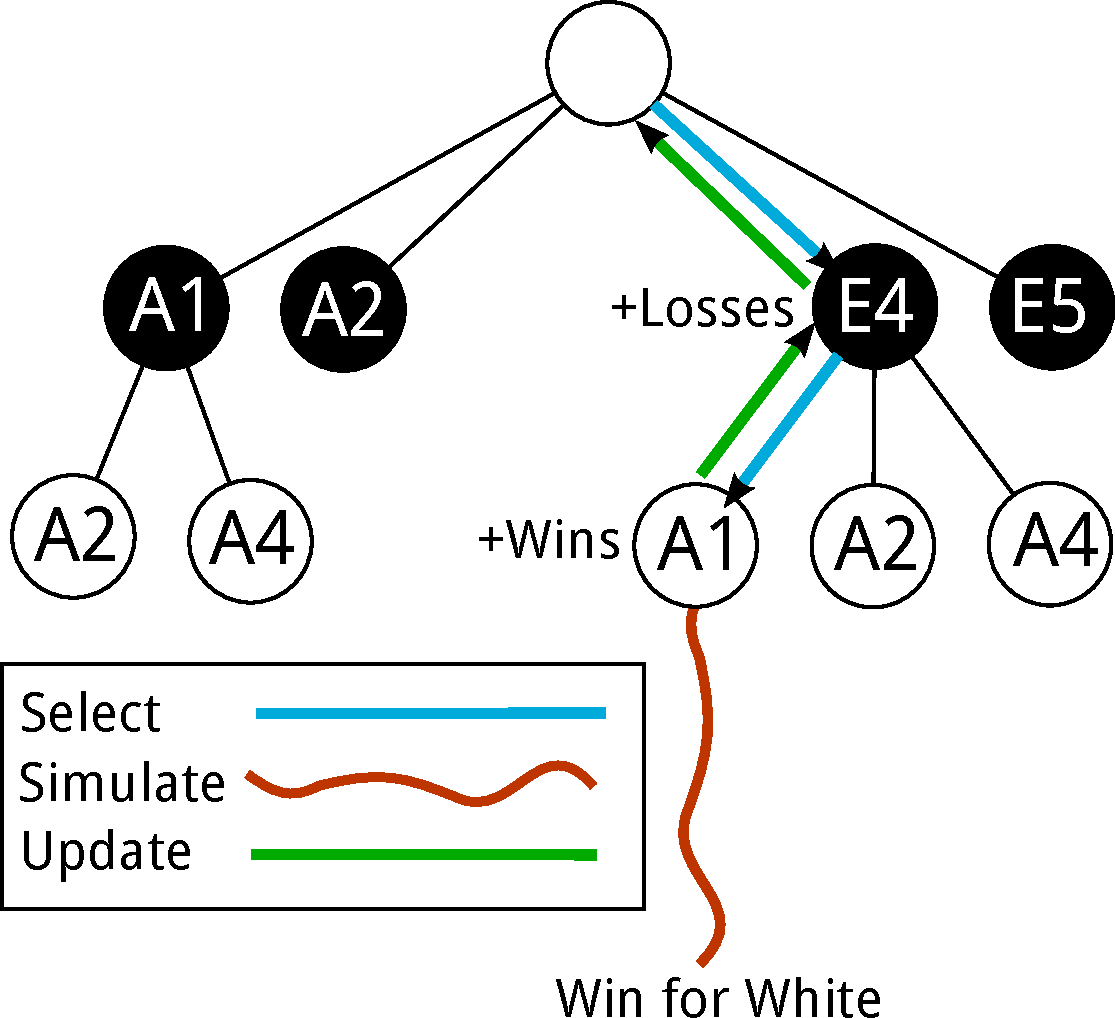
\includegraphics[width=2.5in]{graphics/tree.pdf}
	\end{center}
	\caption{Partial MC Search Tree}
	\label{fig:tree}
\end{figure}

The basic Monte-Carlo technique for computer Go was proposed by Br\"{u}gmann~\cite{brugmann1993monte}. His program \emph{Mango} effectively used a ``flat'' search tree (1-ply) and simply ran simulations from each candidate move to estimate its value. 
Later MCTS techniques use Monte-Carlo simulations to grow a partial search tree. 
The UCT algorithm was developed alongside MCTS to direct the growth of the search tree~\cite{gelly2006exploration}. 
At any point, the search can be stopped and the current state of the tree used to select a move to play. 


All nodes in the tree correspond to a fixed board position, i.e.~the occupancy state of the board and which player is next to move. 
Nodes also have statistics associated with their position:  the number of winning simulations performed that used the node, and the total number of simulations that included the node. 
For each simulation the algorithm will start at the root node, recursively traverse the (partial) tree until it reaches a leaf node.
The simulation continues from the position represented by this leaf node until a winner is determined.
The result of the simulation is used to update the statistics at nodes in the tree
(see Listing 1).
If the leaf node has been visited enough times (50 in our case\footnote{Lower numbers promote accurate exploration at the cost of larger trees and increased computation. Our choice of 50 is somewhat arbitrary, values from 1 to 100 are used in UCT programs on the CGOS Computer Go Server\cite{cgosbots}.}), then it is expanded and nodes for all possible moves from 
that position are added to the search tree.

The effectiveness of MCTS depends on three policies:
\begin{itemize}
\item{The \emph{child-selection} policy recursively traverses the tree, selecting promising moves for further exploration.}
\item{The \emph{continuation} policy randomly or semi-randomly ``plays out'' the game from a leaf position in the tree until a final position.}
\item{The \emph{update} policy modifies the win/loss statistics of nodes based on the simulation results, and determines when to grow the search tree.}
\end{itemize}

Gelly and others have shown that using heuristics in both the child-selection and continuation policies 
can prove extremely beneficial~\cite{gelly2006modification,gelly2008achieving} for Go.
However, this requires expert knowledge (heuristics) that is hard to obtain or not available for some games (particularly new games). 

Figure \ref{fig:tree} shows a partial Monte-Carlo search tree for the given position. In the example, the child-selection policy visited the node for \texttt{Black E4}, then \texttt{White A1}. 
The continuation policy ran, completing the game from the positiion with \texttt{E4} occupied by \hblack\ and \texttt{A1} occupied by \hwhite.
This resulted in a loss for \hblack. 
The update policy updates all nodes along the visited path, incrementing the wins for \hwhite\ moves and incrementing the losses for \hblack\ moves.

\begin{lstlisting}[float,frame=single,language=Pascal,caption=MCTS Algorithm Pseudocode]
function search(root):
  for i in range(simulations):
    simulate_from (root)

function simulate_from(node) returns outcome
  if node is leaf
    outcome =  continue_from (node)
  else:
    child = select_child (node)
    outcome = simulate_from (child)
  node.visits++
  if outcome is  node.player win
    node.wins++
  if (node.visits ==  50) expand (node)
  return outcome
\end{lstlisting}

\subsection{Child Selection Policy}
The \verb+select_child+ function defines the child selection policy. It must return the child of the given node to step into next. 
In general, child selection must trade off between \emph{exploitation} and \emph{exploration}. 
It is important to ``exploit'' those child nodes with high win-rates, both
to discover possible weaknesses and to obtain highly accurate win-rate estimates. 
Simultaneously, a child with a low number of visits must also be explored since a low win-rate
could be due to a few unlucky simulations.
This exploration/exploitation tradeoff is related to a variance reduction problem.  
We want very low variance on the estimates for the good moves in order to maximize the chances of making the best move.
On the other hand, if the variance of a seemingly poor move is very high, then there is a significant chance that that move could actually be very good.

One way to balance this exploration/exploitation trade-off is the Upper-Confidence for Trees algorithm (UCT). 
UCT incorporates the win-rate of a child with a term that increases in value as the ratio of the child's visits to its parents decreases. 
Eventually, no matter how bad the estimated value of a position is, it will be re-visited and the estimate updated. 
UCT has several variations, but the ``pure'' version has been proven to eventually yield the correct minimax value of a position, given an infinite number of simulations~\cite{gelly2006exploration}.

The UCT priority of a child node is:
\[
	\texttt{child.winrate} + C*\sqrt{\frac{\log{(\texttt{parent.visits})}}{\texttt{child.visits}}}.
\]

The \emph{exploration coefficient}, $C$, can be varied to increase or decrease the level of exploration versus exploitation. Note that a very low value will yield a function that relies almost exclusively on the estimated win-rate of a position, while a high value will visit nodes more equally, placing less emphasis on the estimated value.

\subsection{Continuation Policy}

The \verb+continue_from+ function plays out the rest of the game from the current position. 
The simplest policy, which we call the \emph{default policy},
 plays uniformly at random from the legal moves until the game ends (in Hex, when one player has a winning path). 
The continuation policy has a large effect on the strength of the MCTS player.
In fact, one of the top Go engines, MoGo, uses a near-zero exploration coefficient in its child selection policy,
putting most of the control of the search in the hands of the continuation policy~\cite{gelly2007combining}.
Initial research in MCTS Go players focused on using a strong continuation policy, with expert-derived heuristics to select the next move~\cite{chaslot2010adding}. 
The top computer Go programs all have complex hand-crafted policies with rules to examine the current position and select a ``good'' move to play, possibly with a stochastic choice between several candidates. 
Only when none of the rules match do they fall back to a uniform random move. 
It was quickly found that building a stronger continuation policy does not guarantee better performance when used in the full tree search~\cite{gelly2006modification}. 
In other words, when the continuation policies are used as players, the relative strengths of the continuation policies are poor predictors
of how well the MCTS algorithms relying on these continuation policies will perform.
This surprising result may be due to stronger continuation policies under-exploring the search space.
In any case, this means that hand crafting an effective continuation policy requires benchmarking and frequent tests of the entire
MCTS system as small changes to the simulation policy can have unpredictable effects on overall performance.
This illustrates the need for automated systems for tuning the continuation policy.

Another constraint on the continuation policy is its speed.  
MCTS algorithms require large numbers of random simulations to compute accurate statistics and select good moves, therefore the continuation policy must be not be overly complex and implemented efficiently.

\subsection{Update Policy}
Once a simulation is finished, the result is used to update the search tree.
Basic MCTS systems updated the win and visit statistics only along the traversed path.
It was quickly discovered that more aggressive update strategies are often profitable.
One simple example is the All-Moves-As-First (AMAF) heuristic~\cite{brugmann1993monte}
that exploits the fact that moves played in a simulation could have been played in any order. 
Thus, a move deep in the simulation could be fictitiously treated as the ``first'' move from an intermediate position. 
In addition to updating the statistics of the nodes in the path, all children of nodes on the path corresponding to moves made later
in the simulation also have their AMAF win and visit counts updated. 

Several methods can be used to blend the AMAF results with the ``pure'' results, such as a weighted average.
Other blending functions include Cutoff and Rapid Action Value Estimation (RAVE)~\cite{chaslot2008progressive}. 
Helmbold and Parker-Wood (2009) have a summary of the various update policies and blending methods, along with experimental results showing marked improvement over the baseline of pure UCT~\cite{helmbold2009all}. 
One noteworthy conjecture is that there is no ``silver bullet'' update policy. If the simulation policy is random and unbiased, the AMAF updates might be similarly unbiased. However, a simulation policy that preferentially plays certain moves might have an unpredictable effect on which nodes receive AMAF updates. This can then propagate to which nodes are selected during the UCT selection, and have chaotic effects on the search as a whole. 

Our Hivemind experiments use only the basic update policy, updating win and visit counts for only those nodes on the traversed path.

The tree update policy also determines how the partial search tree is grown.
Generally, systems will add the possible children of a leaf to the tree after the leaf has been visited a sufficient number of times.
This number is a parameter in Hivemind, and our experiments have set it to the (untuned) value of 50.

\section{The Hivemind System}\label{hivemind}

Hivemind is a system that learns to play abstract strategy games on a regular board. 
The system consists of three modules: the evolutionary learning process, a Monte-Carlo based UCT search tree implementation, and a ``Game Tracker interface'' used by the tree search to maintain game state information. 
The design was influenced by Fuego, although Hivemind is written in a different language (Google's Go~\cite{golang}). 
In particular, the tracker interface is very similar to Fuego's subclassing system for implementing multiple games~\cite{Fuego}. 
Hivemind's tracker interface is currently implemented for the games of Hex, Go, and Tic-Tac-Toe. 
The major contribution of Hivemind is the integration of evolutionary learning to automatically learn appropriate continuation policies.
Preliminary work tried learning with particle swarm optimization, but we found that evolution strategies gave
superior results.

Using evolution strategies to learn continuation policies requires that the continuation policies are encoded as vectors.
We first describe this encoding.  Section~\ref{s:tracker} describes the Game Tracker module, and Section~\ref{s:es} describes the
use of Evolutionary Strategies.

\subsection{Continuation Policies and Local Patterns}
\label{s:policies}

Hivemind uses local patterns around the previous move to bias the random continuations.
Responding to an opponent's threat is often necessary in cutting and connecting games
and local patterns around the last move can be efficiently evaluated, allowing for efficient simulation.
Strong MCTS Go programs like MoGo~\cite{gelly2006modification} use hand-crafted local patterns to direct their  continuation policies.

Each empty location around this last move is a candidate local response, and a pattern database gives each of these candidates a
weight indicating its relative importance.
During a continuation play-out, a candidate local response is selected with probability proportional to its weight.
Figures \ref{fig:localpattern} and \ref{fig:encoding} show graphically how a local patterns can be mapped to an integer. 
The orange marker denotes the last move played. 
In Hex there are less than $2 * 4^6=2^{13}$ possible local patterns, and 
assigning a weight to each of these patterns creates a continuation strategy.
Thus the continuation strategies we consider correspond to an array of $2^{13}$ weights, one for each local pattern.

In the example shown in figure \ref{fig:localpattern}, the sum of the three weights is 11. Thus, vertex A will be selected with probability $P(A) = \frac{6}{11} \approx 0.54$. 
B will be selected with $P(B) \approx 0.27$ and C with $P(C) \approx 0.18$. 
Note that $P(A)+P(B)+P(C) = 1$ so one of A, B, or C will be selected. 

\begin{figure}
	\begin{center}
	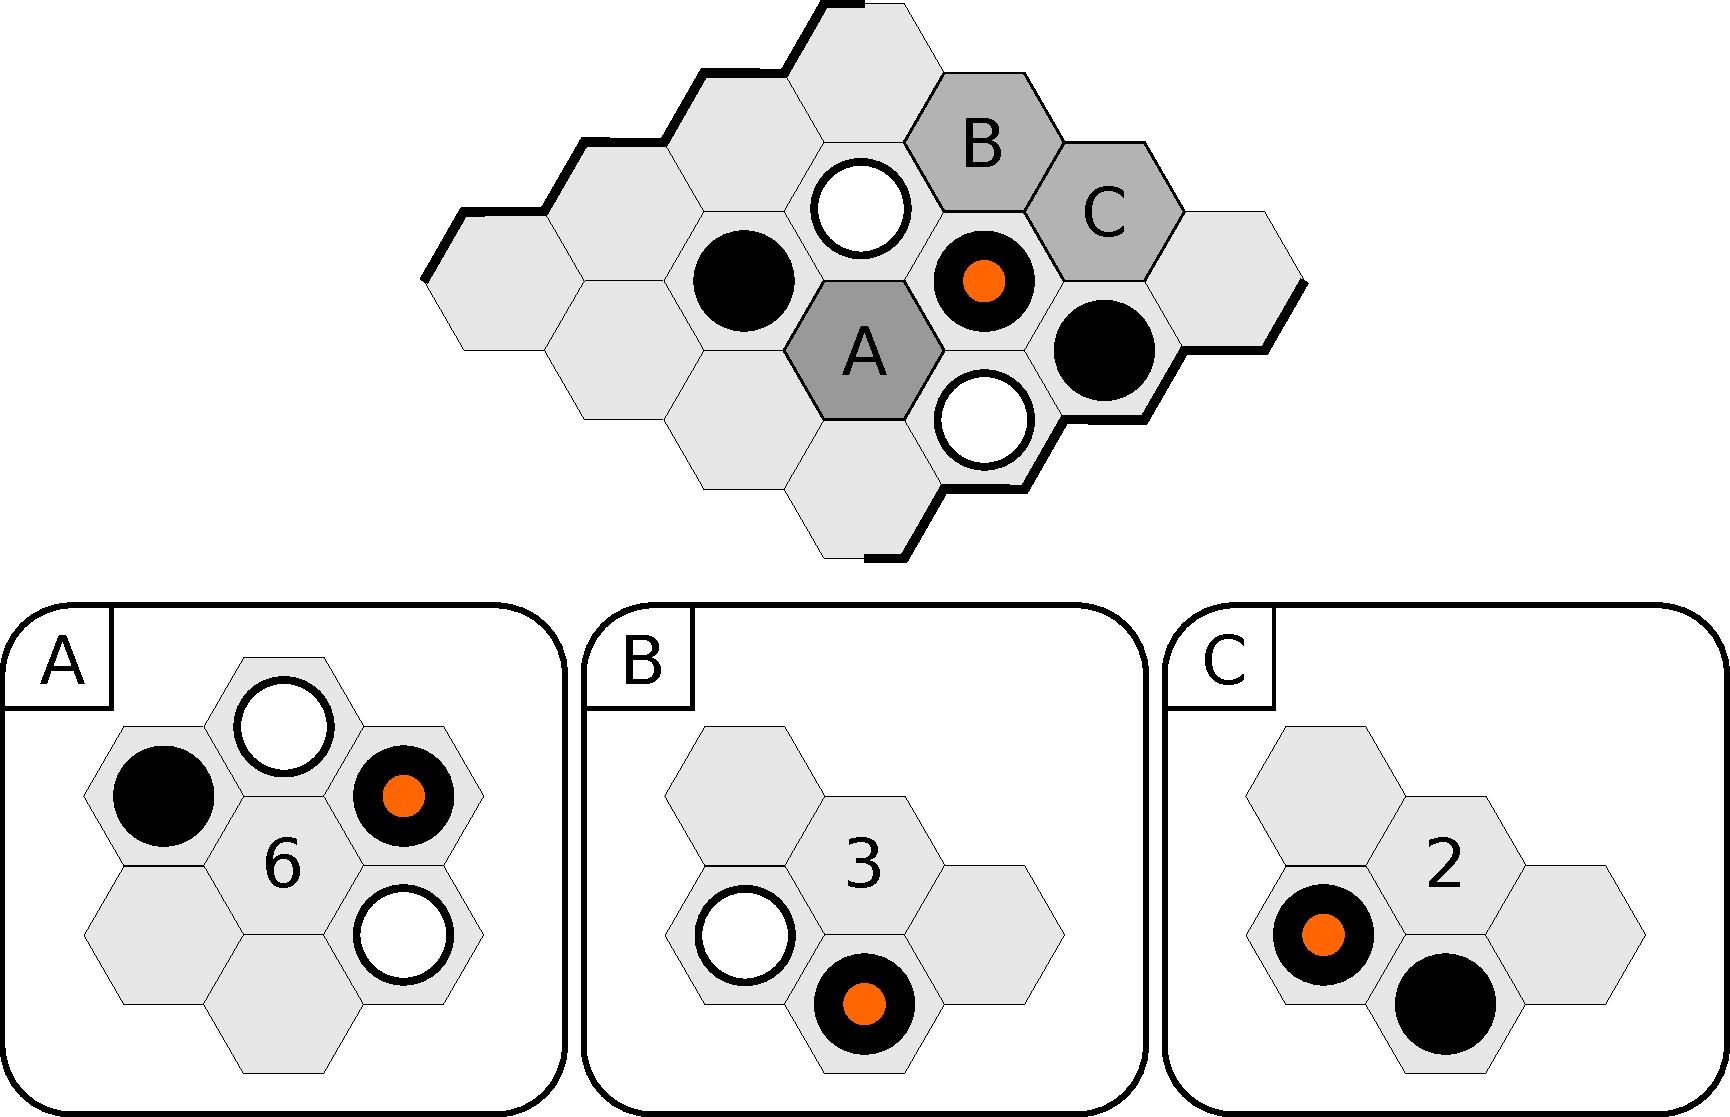
\includegraphics[width=2.85in]{graphics/local-pattern.pdf}
	\caption{A 4x4 board with the 3 patterns shown around \hblacks\ last move. Example weights are shown in the center vertex.}
	\label{fig:localpattern}
	\end{center}
\end{figure}

\begin{figure}
	\begin{center}
	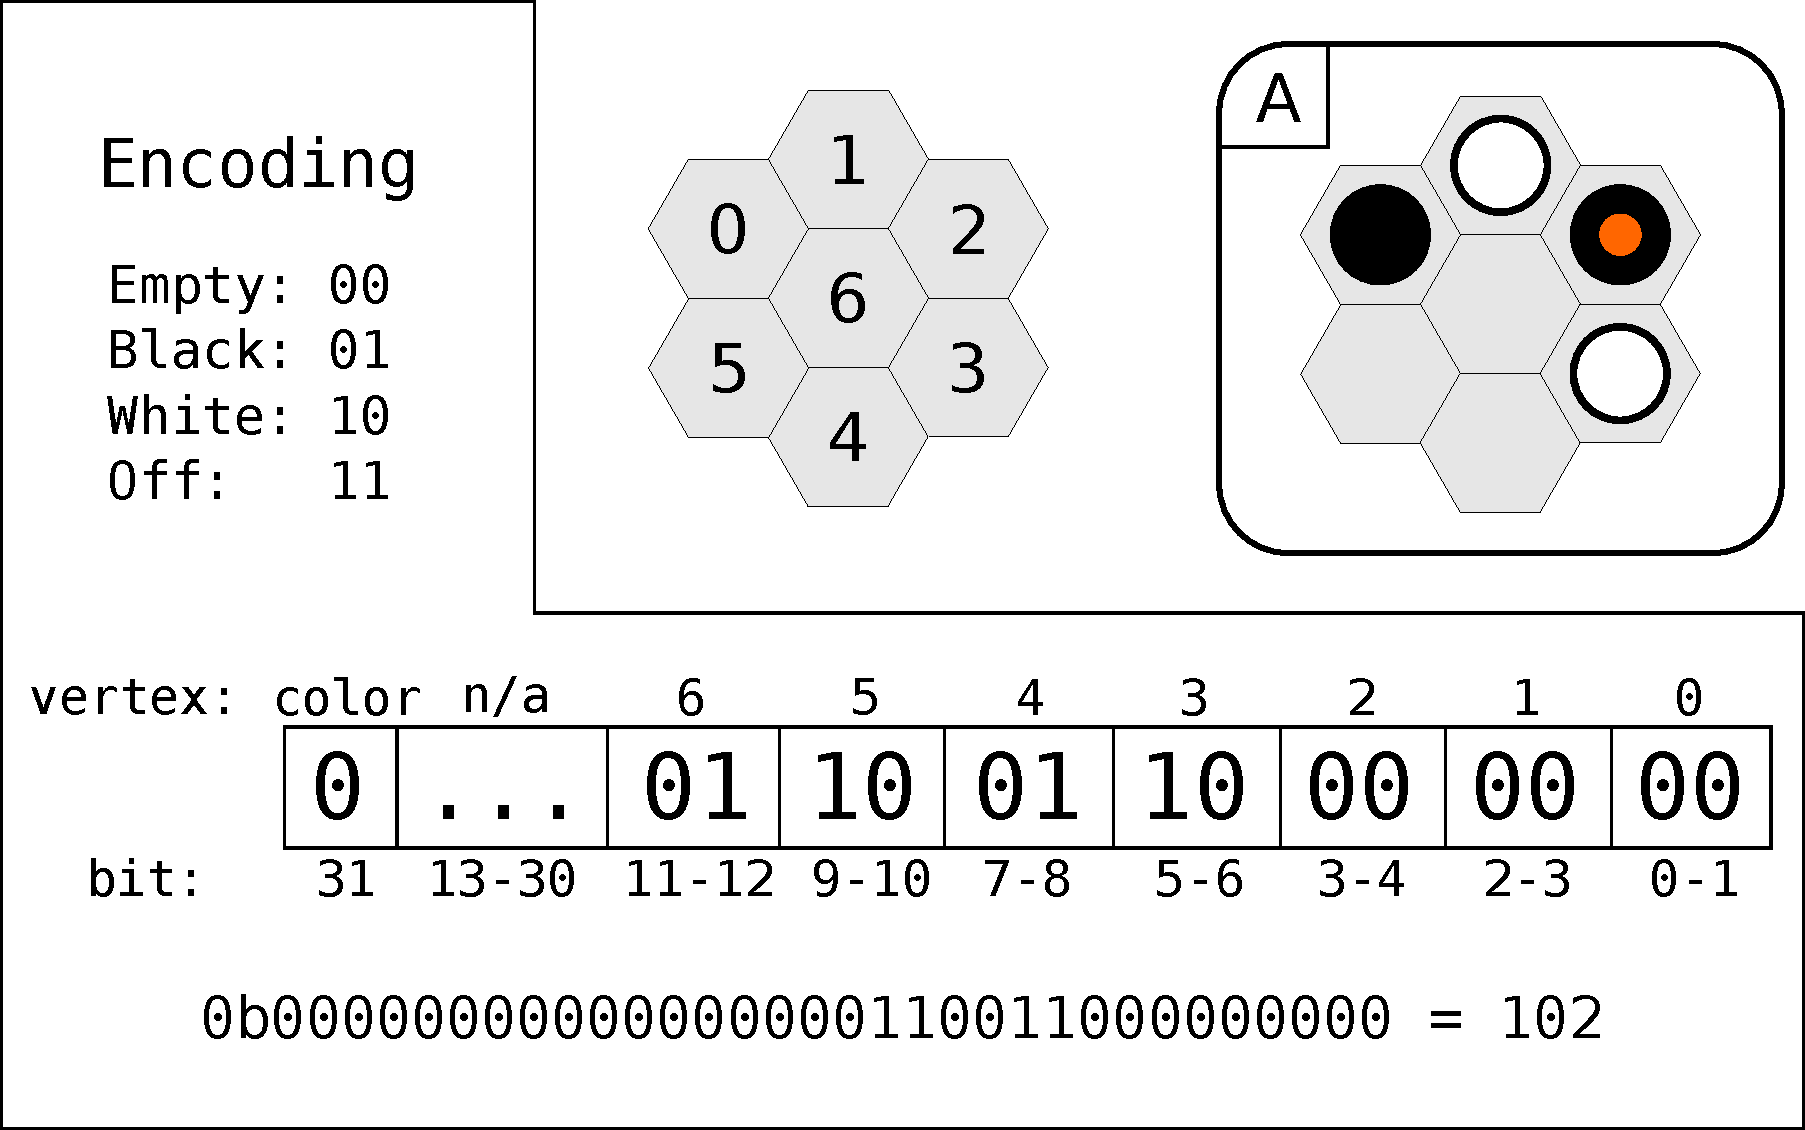
\includegraphics[width=3.25in]{graphics/weight-pattern-map.pdf}
	\caption{The encoding from pattern A to a 32-bit integer. Using the weight from figure \ref{fig:localpattern}, the real value 6 would be stored at position 102 in the weight map.}
	\label{fig:encoding}
	\end{center}
\end{figure}

A local pattern can assign a candidate move a weight of 0. If so, it will never be selected using the local response policy. 
If all patterns adjacent to the last move have weight 0, or if all adjacent vertices are already occupied, 
the continuation policy makes a move at random from all legal possibilities.

Although conceptually an array with $2^{13}$ entries, Hivemind implements continuation strategies as
32-bit hashmaps.  
The additional overhead is modest and the larger hashmaps  have space for additional properties (such as distance to a side).
Note that in Figure~\ref{fig:encoding} the encoding includes a color bit in the 31st position. This denotes the color to play (either \hblack\ (1) or \hwhite\ (0)). 
This bit is important because \hblack\ and \hwhite\ have different goals -- they are trying to connect along different diagonals. 
By using a reflection and flipping colors, one position can be translated into a symmetric  position for the opposite color. 
We experimented with this approach, but it proved more troublesome than beneficial.

Note that many kinds of local hand-coded patterns (like those used by MoGo \cite{gelly2006modification} for Go) can be expressed using the Hivemind encoding system.

\subsection{Hivemind Game Tracker module}
\label{s:tracker}

The Game Tracker module allows real games to be played via Monte-Carlo Tree Search.
Its design was influenced by Fuego~\cite{Fuego},  and the Game Tracker interface is very similar to Fuego's subclassing system for implementing multiple games.
Note that playing a single \emph{real game} involves playing millions of  \emph{simulated} games when
moves in the real game are chosen using Monte-Carlo Tree Search.
Part of the Game Tracker's responsibility is to maintain the 
current simulation.
The Game Tracker also stores the continuation policies of the two players as well as both
the real-game board state and the board state in the current simulation.
Note that the player making the move in the ``real game" uses their continuation policy for both players in the simulated games.


The MCTS  module is a simple 
generic implementation of Monte-Carlo Tree Search, using the UCT algorithm for child selection
(see Section \ref{mcts}).
The MCTS module uses the Game Tracker to keep track of the simulated game state 
as it runs simulated games and expands the search tree.
The MCTS module is only about 600 lines of source code. 
Using some extra information from the Game Tracker,  
the MCTS module can be configurable to use RAVE and AMAF heuristics to 
update multiple nodes using the results of a single simulation.  

The Game Tracker uses the policy weights for the players to implement the appropriate continuation policy and complete simulated games. 
It also implements the three baseline continuation policies described in Section~\ref{s:policies}.
Completing simulated games quickly is critical, as more simulations-per-second generally results in better move selection. 
This emphasis on speed is why the tracker uses a monolithic \texttt{Playout} function
to implement continuation policies.
Many games have optimizations that can be performed in this \texttt{Playout} function that the search tree is unaware of. 
For example, the Hex tracker initializes a randomized list of empty positions so default policy move selection is a O(1) operation. 
This exploits the fact that in Hex, any empty location is a legal play. 
This is not the case for Go, so the Go engine uses other optimizations for fast random move selection.

The Game Tracker module uses an interface that is easily extendible to other games. 
In addition to the \texttt{Playout} function, the Game Tracker provides the following functionality.

\begin{enumerate}
\item A single function, \texttt{Play(color, vertex)}, is used by the search tree to make a move in the simulated game.
\item The \texttt{Legal(color, vertex)} function is used to query the legality of a given move in the simulated game. 
The MCTS module uses this when the tree is gown as each time a leaf node is expanded,
one child is added for each legal move from the leaf node's state.
\item The \texttt{Winner()} function is used to determine the current winner of the game. 
	A special \texttt{Empty} player is returned if the game has not finished.
\item The \texttt{WasPlayed(color, vertex)} function provides information required for the AMAF heuristic.
\end{enumerate}

A few extra functions also provide for debugging by pretty-printing the tracker's internal state.

The Game Tracker interface provides a simple definition of what is needed for a game to use the MCTS+UCT framework. 
In particular, Hivemind is well suited for 2 player placement games with perfect information. 
Since node expansion uses the \texttt{Legal(color, vertex)} function to find all legal children,
Hivemind is not constrained to games with regular boards.

\subsection{Evolution Strategies}
\label{s:es}

Hivemind implements evolution strategies to learn good continuation policies.
Evolution strategies (ES) is a collection of algorithms that operate on real-valued vectors. 
More information on evolution strategies and evolutionary learning in general can be found in Eberhard and Shi's excellent textbook \emph{Computational Intelligence: Concepts to Implementations}~\cite{eberhart2007computational}. 
The Evolution Strategies article on Scholarpedia.org also provides a good introduction to the topic~\cite{Beyer:2007}.


Our implementation of ES works as follows.
\begin{enumerate}
\item An initial population (we use 30 individuals) is randomly generated. 
Each individual is represented by its vector of $2^{13}$ local pattern weights 
(each pattern weight is randomly chosen from $[0 .. 100]$)
and a strategy parameter $\sigma$ that controls how fast it evolves.
During assessment, the individual will also be assigned a real-valued ``fitness'' attribute.
\item The algorithm iterates the following with each iteration forming one ``generation'':
	\begin{enumerate}
	\item From the 30 parents, generate 35 children.
		\begin{enumerate}
		\item Each child is created by randomly selecting 2 parents and then 
		averaging the parents' local patten weight vectors and strategy parameters.
		\item	The child's strategy parameter $\sigma$ is \emph{mutated} to $\sigma e^{ {\cal N}(0,\tau^2)}$
			(see below).
		\item Each local pattern weight of the child is mutated by adding a random variable drawn from the Normal Distribution
		${\cal N}(0, \sigma^2)$.
		\end{enumerate}
	\item The best 5 performing parents are propagated through without mutation.  This is commonly done to preserve well-performing solutions. 
	\item Evaluate the fitness of the new pool of 40 individuals, and keep only the top 30 as parents for the next generation.
	\end{enumerate}
\end{enumerate}

The numbers of:  individuals starting generations, children generated, and good parents kept without mutation
were picked arbitrarily, and do not have deep significance.

\subsubsection*{Mutation of $\sigma$}
Note that $\sigma$ is multiplied by a positive factor at each time step, and can never reach zero. 
The ``learning rate" $\tau$  can be scaled up or down to increase or decrease the variance of $\sigma$, a high values will give more mutation, low values less. 
We use an initial $\tau = \frac{1}{\sqrt{2^{13}}}$ (recall that there are $2^{13}$  pattern weights) and decrease $\tau$ to zero 
as the number of generations approaches a set maximum (100 in our case). 
This forces the algorithm to converge, though not necessarily to an optimal solution. 
This choice of $\tau$ is driven by experimental literature suggesting it works in many cases~\cite{Beyer:2007}.

\subsubsection*{Fitness Evaluation}

Every generation, each individual plays $n=5$ complete games against opponents chosen  randomly from the current population.
Opponents are drawn with replacement, so a given individual could play the same opponent more than once each generation. 
At the beginning of each game, one of the two players is randomly chosen to play \hblack, the other to play \hwhite. 
A swap-safe move was used to play the first move to greatly reduce the first-mover advantage. 
The winner of each game receives 1 point added to their fitness, the loser has 1 point deducted from their fitness.
This means that individuals will be evaluated on about $10$ games, but the exact number depends on how often they are
chosen as opponents.

\section{Results and Conclusions}\label{results}

We experimented with Hivemind and evolution strategies to answer the following four questions:
\begin{enumerate}
\item Do learned continuation policies have an advantage over the three baseline MCTS polices?
\item Are the results of evolution strategies learning stable and predictable?
\item How effective are the learned policies against world-class competitors?
\item Do the learned continuation policies generalize well to other board sizes?
\end{enumerate}

To train the learned policy we used the evolution process as described in Section~\ref{s:es} was run for 100 generations.  
Each evaluation game was played on a 7x7 board and used 1000 simulations per move in the fitness evaluation games. 
The individual from the 100th generation having the highest fitness was selected as the \emph{learned continuation policy}.
This learned continuation policy, as well as the three basic continuation policies described in Section~\ref{s:policies}, were coupled with
a slightly modified UCT child selection policy that included the variance term suggested by Gelly 2006~\cite{gelly2006exploration} and a
pure update policy, where only those nodes directly in the path traversed by UCT are updated with the result of a simulation.
Matches were run using the Gomill software~\cite{gomill}. 
Gomill required no modification to work with Hex playing programs.  

\subsubsection*{Benefits of learned policy}
In principle any player could be used to evaluate the effectiveness of learning.   
We used a round-robin tournament between the learned policy and the three following continuation policies that were easily implementable in Hivemind.

\begin{description}
	\item[Default] - The next move is chosen uniformly at random from the set of all legal moves.
	This policy corresponds to setting all of the weights to 0 in our encoding .
	\item[Uniform local] - The next move is chosen uniformly at random from the empty locations adjacent to the last move.
	If no legal move exists on these 6 points, then the move is chosen uniformly from the set of all legal moves 
	(i.e. using the default policy).  This policy corresponds to setting all the weights to 1.
	\item[Uniform local with ``tenuki''] - The tenuki (Japanese for  ``play away'') variant is a mixture of the Default and Uniform local policies.  
	With probability 5/6 the move is chosen with the Uniform Local policy and with probability 1/6 it is chosen with the Default policy. 
\end{description}

Each match consisted of 200 games on a 7x7 board where the first player alternated was forced to start with a
swap-safe\footnote{A swap-safe first move is a neutral or mediocre move by the first player in an attempt to eliminate the first-player advantage.  This is similar to the \emph{Komi} rule in Go.  We used C4 in our 7x7 games and C8 in the 11x11 games.}
move.
Each player was allowed 10,000 simulations per move and the results are shown in Figure~\ref{fig:results}.

\begin{figure}
	\begin{center}
		\begin{tabular}{c | c c c}
		& \multispan{3}{\hfil opponent \hfil} \\
		 player & default & uniform & uniform (tenuki) \\
		\hline
		uniform & 70.50\% & & \\
		uniform (tenuki) & 61.00\% & 50.00\% & \\
		learned & 90.00\% & 84.00\% & 86.00\% \\
		\end{tabular}
	\caption{All-play-all tournament of the 4 Hivemind variants. Each element is the percent win-rate of the row variant versus the column variant.}
	\label{fig:results}
	\end{center}
\end{figure}

The learned policy is the decisive winner, winning almost 90\% of its games.
This shows the clear benefits of automatically learned weights over the default continuation policies.
We originally thought that the addition of a tenuki probability would add beneficial diversity to the continuation searches, but
it has little or no improvement over the uniform local policy.
As expected, uniform local play significantly improves upon the default (random selection over all legal moves)  continuation policy. 

\subsubsection*{Stability of Evolution}

A natural concern is that the evolution strategies could have large variations in their end results and our first learned policy was just a ``lucky'' happenstance. 
To protect against this, we re-ran the learning process described above another 9 times, creating a total of 10 different learned continuation policies.
We then played 200 game matches between each of the resulting policies and the default policy using the above protocol.
The following table gives the resulting win-rates for the learned policies.

\medskip

\centerline{
\begin{tabular}{c c c c  c c c c  c c c}
\multispan{10}{\hfil Winning \% for Learned Policy vs. Default \hfil} \\
1 & 2 & 3 & 4 & 5 & 6 & 7 & 8 & 9 & 10 \\
91 & 90.5  & 90.5  & 87.5  & 90.5  & 93.5  & 93 & 91.5  & 87 & 92.5 
\end{tabular}
}

The 10 learned policies were tightly clustered with a mean of 90.75\% and a standard deviation of only 2.14\%.
This surprising result indicates that the evolutionary process is far more stable than we expected.

\subsubsection*{Comparison against MoHex}

A potential problem with self-learning is that the system might only be learning how to exploit the weaknesses of its competitors, and not making a general improvement in playing strength.
We use ``general playing strength'' in an intuitive sense -- we want to avoid focusing on
particular ``tricks'' that are only effective against the algorithms in the current population.
Although improvement against the three baseline opponents gives some evidence against this over-specialization, 
we perform further comparison against a strong outside control. 
For this, we used the MoHex program from the University of Alberta, compiled and run with its default settings~\cite{mohex}.
The optimization and domain expertise in MoHex make it a very strong  competitor --  MoHex has won the computer Hex world championships in 2008, 2009 and 2010.

In the 7x7 matches against MoHex, 
MoHex played with the default time limit of 10 seconds per move while the Hivemind programs again used
10,000 simulations per move. 
MoHex uses some of its time to perform game theoretic search and pruning before the Monte-Carlo phase. 
The pre-search can also discover ``must-play'' moves that will be immediately played in lieu of the MCTS. 
Although the time controls are not directly comparable, we did track CPU seconds per game.
MoHex used about 35 CPU seconds per game while the Hivemind programs were a bit faster.
Since we were unable to force MoHex to play a particular first move, all games had the 
Hivemind variant moving first with the swap-safe move.  
The Hivemind win percentages (400 game matches) and average CPU seconds used against MoHex are given below.

\medskip
\centerline{
\begin{tabular}{lccc}
& Learned policy & Uniform local & Default policy \\
win \% & 42\% & 26\% & 11.75\% \\
cpu secs & 20.34 & 15.79 & 13.3 
\end{tabular}
}

As expected, the learned policy does significantly better against MoHex than the other policies,
with the Learned policy winning above 40\% of its games (the results for the other 9 learned policies are similar,
with win rates from 39\% to 47\%).   
The good performance against MoHex is a little surprising, and could be due to the relatively small board size and/or 
a swap-safe move that favors the first player (after any first move, one of the players will have a forced win).
Despite this, the superiority of the learned policy over the baseline ones is dramatically evident.

\subsubsection*{Generalization across board sizes}

The time required to learn greatly depends on the boardsize used. For training, a boardsize of 7x7 was chosen as a tradeoff between computation time and the game's deepness and subtlety.
We now examine how well the policy learned on 7x7 boards generalizes to larger boards. 
We played 200 game matches on 11x11 and 13x13 boards between the learned policy and the 
default and uniform local policies.  
Because of the increased boardsize, each player used 100,000 simulated playouts per move. 

\centerline{
\begin{tabular}{c | cc cc}
 & \multispan{2}{\hfil default \hfil} & \multispan{2}{\hfil uniform local\hfil} \\
 & 11x11 & 13x13 & 11x11 & 13x13 \\ \hline
 learned win \%	& 92.5 \% & 94 \%  & 88.5\% & 85\% 
 \end{tabular}
}

The policy learned on a 7x7 board provides results that can generalize to larger boardsizes. 
In fact, the policy's win rate increases on the larger boards (but not significantly).
This generalization is especially useful because of the exponential increase in computational time required to play games for evolutionary learning when learning on larger board sizes.

On larger boards the learned policy's superiority over the baselines is also evident against MoHex.
The following table gives the results of 200 game matches on 11x11 boards between Hivemind policies (moving first in a swap-safe location, 100,000 simulations per move) and MoHex.

\centerline{
		\begin{tabular}{c  | c c c}
		& &	Hivemind  & Hivemind \\
		Hivemind & Opponent & Win-rate & Relative CPU \\
		\hline
		Default & MoHex & 0.5\% & 510\% \\
		Local & MoHex & 0.0\% & 545\% \\
		Learned & MoHex & 11\% & 620\% \\
		\end{tabular}
}

The learned policy provided 22 of the 23 wins against MoHex.
Whereas the Hivemind programs were faster on the 7x7 boards, MoHex's optimizations allow it to use only 1/5 to 1/6 the CPU time on the larger board. Note that the pattern lookup required by the learned weights slightly increases the time per simulation.

\subsubsection* {Conclusions}
With infinite time, an unbiased playout policy can find the true minimax value of a position in the game of Hex. 
In practice, both resources and time are finite. 
Bias in the playout policy is extremely useful for improving the overall quality and performance of a Monte-Carlo Tree Search and evolutionary learning can provide a substantial performance boost over naive patterns. 
We showed how self-play and evolution can automatically learn good weights, without requiring expert knowledge or manual tuning. The learning process can be done offline, and the final result requires little overhead.

It is worth emphasizing that  the learned continuation policies are coupled with relatively naive update and child-selection polices.  
There is still a large gap between the automatically learned Hivemind policy and current champion programs,
but it remains to be seen how much of this gap can be closed with improved child-selection and update policies.

Source code for the Hivemind Computer Hex/Go player is available at \url{http://github.com/etherealmachine/hivemind}. The included README file has instructions on running the evolutionary learning process and using the results.

\subsection*{Acknowledgements}
We thank David Doshay and the Hierarchical Systems Research Foundation for the use of the their compute cluster. \\

\bibliography{paper}
\bibliographystyle{plain}
\end{document}
